\chapter{Polarised PDFs from DIS and SIDIS}
\label{ch:4}

In this Chapter, we present the first determination of polarised PDFs at next-to-next-to-leading order accuracy based on the MAP methodology, \texttt{MAPpol1.0}. The determination has been carried out including all available data from inclusive and semi-inclusive, neutral current, polarised DIS coming from different facilities. The final result will be a determination of light-flavours quark, antiquark, and gluon distributions at NNLO accuracy. In \secref{sec:4.1} we review the available data sets, and we discuss how pseudodata are generated in the context of the Monte Carlo method. The details of the analysis are discussed in \secref{sec:4.2}. In \secref{sec:4.3} we review the fitting strategy and discuss how the methodologies discussed in \chapref{ch:3} apply in our case. Finally, the \texttt{MAPpol1.0} parton set is presented in \secref{sec:4.4}, together with its stability upon the variation of some theoretical constraints.

\section{Experimental input}
\label{sec:4.1}

We review the experimental data sets used in the determination of the \texttt{MAPpol1.0} parton set, and we present how the uncertainties are taken into account. Then, we show the construction of the artificial ensemble of data points based on the Monte Carlo sampling method.

\subsection*{Data sets}
%%
\begin{figure}[t]
  \centering
  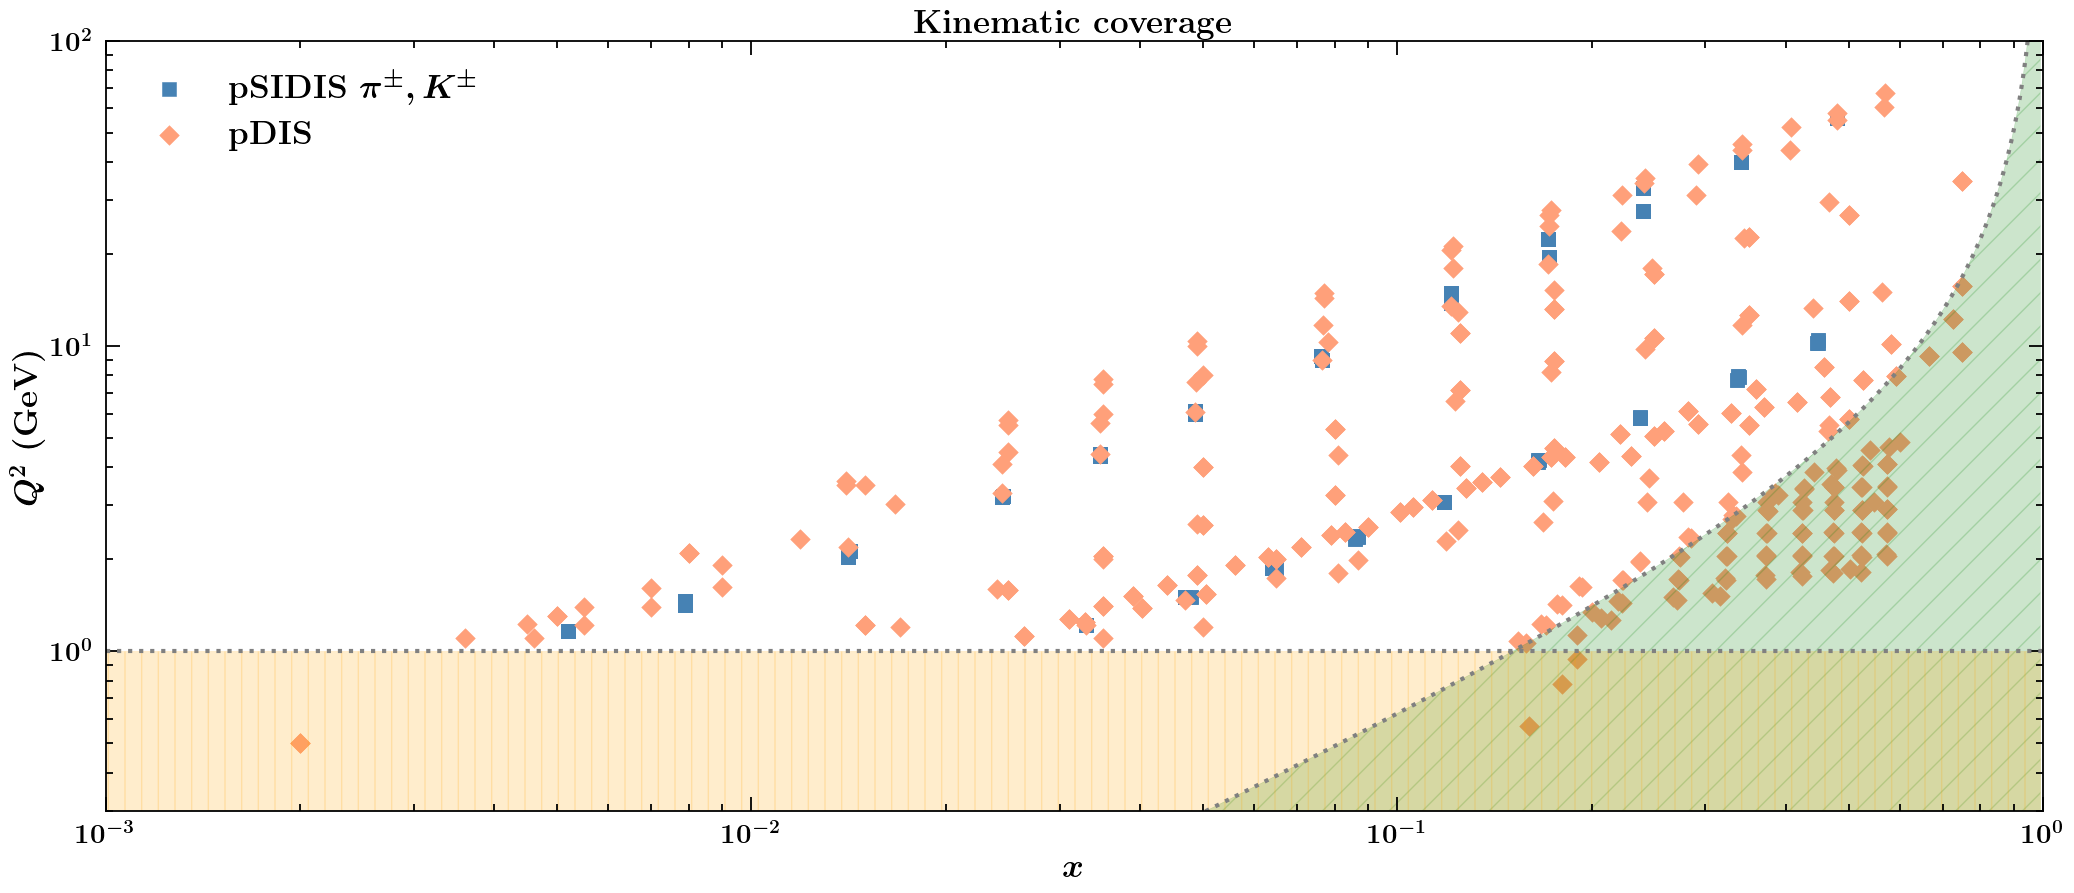
\includegraphics[width=1\textwidth]{kin_cov.png} 
  \caption{\small{Kinematic coverage in the $(x,Q^2)$ plane. The orange- and green-coloured areas represent the cuts in $Q^2$ and $W^2$, respectively.}}
  \label{fig:kin_cov}
\end{figure}
%%
In our analysis, we use inclusive and semi-inclusive lepton-nucleon DIS data coming from different facilities such as CERN \cite{EuropeanMuon:1989yki, SpinMuon:1999udj, COMPASS:2006mhr, COMPASS:2010wkz, COMPASS:2010hwr}, SLAC \cite{E142:1993hql, E143:1998hbs, E154:1997xfa, E155:2000qdr}, DESY \cite{HERMES:2018awh, HERMES:2006jyl, HERMES:1997hjr} and Jefferson Lab \cite{Kramer:2002tt, JeffersonLabHallA:2004tea, CLAS:2014qtg}. For both DIS and SIDIS, the lepton beams are made of either electrons or muons. The targets are either protons or neutrons, and, in some case, deuterons. The main features of the data sets are summarised in Tabs.~[\ref{tab:DIS_data}, \ref{tab:SIDIS_data}], in which we show the number of data points, the kinematic coverage, and the measured observables. The global kinematic coverage in the $(x,Q^2)$ plane is also shown in Fig.~\ref{fig:kin_cov}. \par
The observable that we use in the analysis is the (semi-)inclusive structure function $g_1^{(h)}$. However, some experiments provide its value normalised the unpolarised structure function, that is $g_1^{(h)}/F_1^{(h)}$. Thus, in computing the predictions, we must calculate the unpolarised structure function $F_1^{(h)}$, which introduces an additional dependence on the unpolarised parton set. The unpolarised set of PDFs adopted in the analysis is \texttt{NNPDF\red{which one?}}. We observe that some experiments publish many data tables with different observables, which eventually may be used to reconstruct the structure function of interest (see \textit{e.g.}, Ref.~\cite{Nocera:2014vla}).\par
In order to ensure the reliability of perturbative QCD, we exclude all data points with $Q^2 \leq Q^2_{\T{cut}} = 1 \, \T{GeV}^2$. This cut corresponds to the orange-coloured area of Fig.~\ref{fig:kin_cov}. In addition, we also impose a cut on the squared invariant mass of the hadronic final state $W^2$, in order to remove all the points that may be affected by higher-twist corrections, as discussed in \secref{sec:field_theoretic}. In particular, we will exclude points such that $W^2 \approx Q^2 (1-x)/x \leq W^2_{\T{cut}} = 6.5 \, \T{GeV}^2$. The excluded area  is shown in green in Fig.~\ref{fig:kin_cov}.\par
The resulting kinematic coverage is highly affected by these cuts. Starting from $480$ initially available points, after cuts this number reduces to $N_{\T{dat}}=360$,  -- a reduction of the $\sim 25\%$ respect to the initial points. We observe that the most affected experiments are those performed by Jefferson Lab \cite{Kramer:2002tt, JeffersonLabHallA:2004tea, CLAS:2014qtg}. Indeed, the cut in $W^2$ mainly affects all data points that cover the large-$x$ and small-$Q^2$ corner, which is exactly the region probed by these experiments.\par
Although the coverage of both low- and large-$x$ regions have been improved in recent years, the present situation for polarised data is not comparable with the unpolarised counterpart. This latter provides over than $3000$ data points coming from different processes other than DIS (see \textit{e.g}, Ref.~\cite{Kassabov:2022pps}). Moreover, the accuracy of these points is also better if compared to the unpolarised case. Still, this does not prevent us to perform a global determination, provided a reliable estimation of PDF uncertainties.\par
For each observable listed in Tabs.~[\ref{tab:DIS_data},\ref{tab:SIDIS_data}], the experiments provide information about their uncertainties.
In particular, correlated systematics (multiplicative and/or additive) are only given by E143, E155, EMC, and HERMES, whereas the other experiments only give uncorrelated uncertainties. With this information at our disposal, we can construct the covariance matrix $V_{ij}$ as follows
%%
\begin{equation}
  V_{ij} =  \sigma_{i,\T{unc}} \sigma_{j,\T{unc}} \delta_{ij} + \sum_{\ell=1}^{l} \sigma_{i,\T{corr}}^{(l)} \sigma_{j,\T{corr}}^{(\ell)} \,,
\end{equation}
%%
\afterpage{
\begin{landscape}% Landscape page
  \begin{table}
  \scriptsize
  \centering % Center table
  \begin{tabularx}{1\pdfpagewidth}{llXXXcccc}
  \toprule \toprule
   Experiment    & Set  &  $N_{\T{dat}}$  &  $x_{\T{min}}$  &  $x_{\T{max}}$  & $Q^2_{\T{min}} [\T{GeV}^2]$ &  $Q^2_{\T{max}} [\T{GeV}^2]$ &    $F$    &  Ref. \\
  \midrule
   E142 
        \\       & E142-G1N & $8\,(7)$ & $.035$ & $.466$ & $1.1$ & $5.5$ & $g_1$ & \cite{E142:1996thl} \\
  \midrule
   E143 
        \\       &  E143-G1D  &   $28\,(25)$  &    $.031$       &      $.749$     &    $1.27$                   &       $9.52$                 &  $g_1$    & \cite{E143:1998hbs} \\       
                 &  E142-G1P  &   $28\,(25)$  &    $.035$       &      $.466$     &    $1.27$                   &       $9.52$                 &  $g_1$    & \cite{E143:1998hbs} \\
  \midrule
   E154 
        \\       &  E154-G1N  &   $11$         &    $.017$      &      $.024$      &   $ 1.2$                    & $15.0$                       & $g_1$     & \cite{E154:1997xfa} \\
  \midrule
   E155 
       \\        & E155-A1P   & $24\,(22)$      & $.015$        & $.750$          &  $1.22$                & $34.72$                & $g_1/F_1$          & \cite{E155:2000qdr}
       \\        & E155-A1N   & $24\,(22)$      & $.015$        & $.750$          &  $1.22$                & $34.72$                & $g_1/F_1$          & \cite{E155:2000qdr} \\
  \midrule
   EMC 
       \\        & EMC-G1P    & $10$         & $.015$       & $0.466$       &    $3.5$         & $29.5$                      & $g_1$          & \cite{EuropeanMuon:1989yki} \\
  \midrule
   JLAB E06 014
       \\        & JLAB-A1N   & $6\,(1)$     & $.277$       & $0.548$      & $3.078$    & $3.078$                  & $g_1/F_1$  & \cite{JeffersonLabHallA:2016neg} \\
  \midrule
   JLAB E97 103
       \\        & JLAB-E97-103-G1N & $5\,(0)$ & $.160$ & $.200$ & $0.57$ & $1.34$ & $g_1$ & \cite{Kramer:2002tt}\\
  \midrule
   JLAB E99 117 
       \\        & JLAB-E99-117-G1N-F1N & $3\,(0)$ & $.33$ & $.60$ & $2.71$ & $4.83$ & $g_1/F_1$ & \cite{JeffersonLabHallA:2004tea} \\
  \midrule
   JLAB EG1 DVCS-D 
       \\        & JLAB-EG1-DVCS-G1D-F1D & $44\,(1)$ & $.158$ & $0.574$ & $1.078$ & $4.666$ & $g_1/F_1$ & \cite{CLAS:2014qtg}
       \\        & JLAB-EG1-DVCS-G1P-F1P & $47\,(2)$ & $.154$ & $0.578$ & $1.064$ & $4.115$ & $g_1/F_1$ & \cite{CLAS:2014qtg} \\
  \midrule
   SMC
       \\        & SMC-G1D & $13\,(12)$ & $.002$ & $.48$ & $0.50$ & $54.80$ & $g_1$ &  \cite{SpinMuon:1999udj} 
       \\        & SMC-G1P & $13\,(12)$ & $.002$ & $.48$ & $0.50$ & $54.80$ & $g_1$ &  \cite{SpinMuon:1999udj} \\
  \midrule 
   COMPASS-D
       \\        & CMP07-G1D & $15$ & $.0046$ & $0.567$ & $1.1$ & $60.8$ & $g_1$ & \cite{COMPASS:2006mhr} \\
  \midrule
   COMPASS-P 
       \\        & CMP10-G1P & $17$ & $.0036$ & $.57$ & $1.1$ & $67.4$ & $g_1$ & \cite{COMPASS:2010wkz} \\
  \midrule 
   HERMES97 
       \\        & HERMES-G1N & $9\,(8)$ & $.033$ & $.464$ & $1.22$ & $5.25$ & $g_1$ & \cite{HERMES:1997hjr} \\
  \midrule
   HERMES 
       \\        & HERMES-G1P & $15\,(14)$ & $.0264$ & $.7248$ & $1.12$ & $12.21$ & $g_1$ & \cite{HERMES:2006jyl} 
       \\        & HERMES-G1D & $15\,(14)$ & $.0264$ & $.7248$ & $1.12$ & $12.21$ & $g_1$ & \cite{HERMES:2006jyl} \\
  \midrule
   Total DIS         &    & $335 \, (218)$  & & &  &    &      &      \\
  \bottomrule
\end{tabularx}
  \caption{
    \small
    Experimental DIS data sets included in the \texttt{MAPpol1.0} analysis. For each experiment we show the number of data points before and after (in parenthesis) applying kinematic cuts, the covered kinematic range and the measured observable.
  \label{tab:DIS_data}}% Add 'table' caption
  \end{table}
\end{landscape}}
%%
\afterpage{
\begin{landscape}% Landscape page
  \begin{table}
  \scriptsize
  \centering % Center table
  \begin{tabularx}{1\pdfpagewidth}{llXXXcccc}
  \toprule \toprule
   Experiment    & Set       &  $N_{\T{dat}}$  &  $x_{\T{min}}$  &  $x_{\T{max}}$  & $Q^2_{\T{min}} [\T{GeV}^2]$ &  $Q^2_{\T{max}} [\T{GeV}^2]$ &    $F$    &  Ref. \\
  \midrule
   COMPASS-P 
     \\          & COMPASS-A1P-KA-MINUS & $12$ & $.004$ & $.7$ & $1.16$ & $55.6$ & $g_1^{(h)}/F_1^{(h)}$ & \cite{COMPASS:2010hwr} \\
                 & COMPASS-A1P-KA-PLUS & $12$ & $.004$ & $.7$ & $1.16$ & $55.6$ & $g_1^{(h)}/F_1^{(h)}$ & \cite{COMPASS:2010hwr} \\
                 & COMPASS-A1P-PI-MINUS & $12$ & $.004$ & $.7$ & $1.16$ & $55.6$ & $g_1^{(h)}/F_1^{(h)}$ & \cite{COMPASS:2010hwr} \\
                 & COMPASS-A1P-PI-PLUS & $12$ & $.004$ & $.7$ & $1.16$ & $55.6$ & $g_1^{(h)}/F_1^{(h)}$ & \cite{COMPASS:2010hwr} \\
  \midrule
   COMPASS-D 
     \\          & COMPASS-A1D-KA-MINUS & $10$ & $.004$ & $.7$ & $1.16$ & $32.8$ & $g_1^{(h)}/F_1^{(h)}$ & \cite{COMPASS:2010hwr} \\
                 & COMPASS-A1D-KA-PLUS & $10$ & $.004$ & $.7$ & $1.16$ & $32.8$ & $g_1^{(h)}/F_1^{(h)}$ & \cite{COMPASS:2010hwr} \\
                 & COMPASS-A1D-PI-MINUS & $10$ & $.004$ & $.7$ & $1.16$ & $32.8$ & $g_1^{(h)}/F_1^{(h)}$ & \cite{COMPASS:2010hwr} \\
                 & COMPASS-A1D-PI-PLUS & $10$ & $.004$ & $.7$ & $1.16$ & $32.8$ & $g_1^{(h)}/F_1^{(h)}$ & \cite{COMPASS:2010hwr} \\
  \midrule
   HERMES-P 
     \\          & HERMES-2018-A1P-PI-MINUS & $9$ & $.033$ & $.449$ & $1.22$ & $10.28$ & $g_1^{(h)}/F_1^{(h)}$ & \cite{HERMES:2018awh} \\
                 & HERMES-2018-A1P-PI-PLUS & $9$ & $.033$ & $.449$ & $1.22$ & $10.17$ & $g_1^{(h)}/F_1^{(h)}$ & \cite{HERMES:2018awh} \\ 
  \midrule
   HERMES-D 
     \\          & HERMES-2018-A1D-KA-MINUS & $9$ & $.033$ & $.449$ & $1.21$ & $10.01$ & $g_1^{(h)}/F_1^{(h)}$ & \cite{HERMES:2018awh} \\
                 & HERMES-2018-A1D-KA-PLUS & $9$ & $.033$ & $.449$ & $1.21$ & $10.07$ & $g_1^{(h)}/F_1^{(h)}$ & \cite{HERMES:2018awh} \\
                 & HERMES-2018-A1D-PI-MINUS & $9$ & $.033$ & $.449$ & $1.21$ & $9.97$ & $g_1^{(h)}/F_1^{(h)}$ & \cite{HERMES:2018awh} \\
                 & HERMES-2018-A1D-PI-PLUS & $9$ & $.033$ & $.449$ & $1.21$ & $9.92$ & $g_1^{(h)}/F_1^{(h)}$ & \cite{HERMES:2018awh}\\
  \midrule
   Total  SIDIS        &    & $142$  &      &      &         &     &     &      \\
  \midrule \toprule
   \\[0.5pt]
   Total & & $477 \, (360)$ & & & & & & \\
  \bottomrule
\end{tabularx}
  \caption{
    \small
    Experimental SIDIS data sets included in the \texttt{MAPpol1.0} analysis. For each experiment we show the number of data points before and after (in parenthesis) applying kinematic cuts, the covered kinematic range and the measured observable.
  \label{tab:SIDIS_data}}% Add 'table' caption
  \end{table}
\end{landscape}}
%%
where $i$ and $j$ run over the experimental data points, $\sigma_{i,\T{corr}}^{(\ell)}$ are the various sources of correlated uncertainties, and $\sigma_{i,\T{unc}}$ are the uncorrelated uncertainties. The latter are defined as the sum in quadrature of all uncorrelated sources of statistical $\sigma_{i,\T{stat}}$ and systematic $\sigma_{i,\T{syst}}$ error for the $i$-th point
%%
\begin{equation}
  \sigma_{i,\T{unc}}^2 = \sigma_{i,\T{stat}}^2 + \sigma_{i,\T{syst}}^2 \,.
\end{equation}
%%
Finally, we anticipate that the first moments of the non-singlet triplet and octet distributions $a_3$ and $a_8$, are treated as two additional data points and enter the computation of the $\chi^2$. The values measured from the hyperon $\beta$-decay are \cite{Nakamura_2010}
%%
\begin{equation}
  a_3 = 1.2701 \pm 0.0025 \hspace{10mm} a_8 = 0.585 \pm 0.025 \,.
  \label{eq:a3_a8_values}
\end{equation}
%%
We will further discuss these two points in \secref{sec:4.3}.

\subsection*{Generation of Monte Carlo replicas}
In order to propagate the error from experimental data, we use the Monte Carlo sampling method as discussed in \secref{sec:MAP}. There, the artificial points are obtained by sampling the distributions of experimental data. As a result, we obtain a statistical ensemble of $N_{\T{rep}}$ replicas that reflects the statistical properties of the original data set.%

The key point to observe is that we want the fluctuated points to follow the same distribution of the unfluctuated data. We assume data to be distributed according to a multi-variate Gaussian distribution, whose mean values correspond to the experimental central points and the covariance matrix is constructed as discussed earlier. The $\chi^2$ obtained by comparing the central unfluctuated value $m_j$ with its fluctuated value $f_j$, expressed in matrix form, must then read
%%
\begin{equation}
  \chi^2 = \tran{\vb*{d}} \cdot \vb*{V}^{-1} \cdot \vb*{d} \,,
  \label{eq:chi_fluc}
\end{equation}
%%
where $\vb*{V}$ is the usual $N_{\T{dat}} \times N_{\T{dat}}$ covariance matrix and $\vb*{d}$ is a column vector with $N_{\T{dat}}$ entries defined as
%%
\begin{equation}
  d_j = f_j - m_j \,.
\end{equation}
%%
On the other hand, the $\chi^2$ is also defined as
%%
\begin{equation}
  \chi^2 = \sum_{i=1}^{N_{\T{dat}}} z_i^2 = \left| \vb*{z} \right|^2 \,,
  \label{eq:chi2_normal}
\end{equation}
%%
where $z_j$ are independent, standard normal random variables such that
%%
\begin{equation}
  \langle z_i \rangle = 0 \hspace{10mm} \T{and} \hspace{10mm}  \langle z_i z_j \rangle = \delta_{ij} \,.
\end{equation}
%%
It immediately follows that $\langle \chi^2 \rangle = N_{\T{dat}}$, as predicted by the $\chi^2$ distribution. Now, the covariance matrix, being a symmetric object, admits the so called Cholesky decomposition, that allows us to write
%%
\begin{equation}
  \vb*{V} = \vb*{L} \cdot \tran{\vb*{L}} \,,
\end{equation}
%%
where $\vb*{L}$ is a lower diagonal matrix\footnote{Further details on the Cholesky decomposition can be found in Appendix \ref{app:lin_sys}.}. Thus, the $\chi^2$ in Eq.~\eqref{eq:chi_fluc} can be recast as
%%
\begin{equation}
  \chi^2 = \left| \vb*{L}^{-1} \cdot \vb*{d} \right|^2 \,.
  \label{eq:chi2_Cholesky}
\end{equation}
%%
Collecting Eqs.~\eqref{eq:chi2_Cholesky} and \eqref{eq:chi2_normal} and after a little algebra, one finally obtains the following relation
%%
\begin{equation}
  f_j = m_j + \sum_{i=1}^{N_{\T{dat}}} L_{ji} z_i\,.
  \label{eq:MC_gen}
\end{equation}
%%
We stress that the above expression has been obtained by imposing that the fluctuated data followed the multi-variate Gaussian distribution and that the $\chi^2$ had the correct distribution. Thus, in order to generate an artificial value, one just has to use Eq.~\eqref{eq:MC_gen}, where $z_j$ is randomly extracted from a centred, univariate Gaussian distribution.\par
It is straightforward to show that the fluctuations generated according to Eq.~\eqref{eq:MC_gen} present the same statistical properties of the original data set. In particular, one can show that
%%
\begin{gather}
  \langle f_j \rangle = m_j \,,\\
  \langle f_j f_k \rangle = \langle f_j \rangle \langle f_k \rangle + V_{jk} \,,
\end{gather}
%%
which are the expected relations for a correct generation of a Monte Carlo ensemble.
%
\afterpage{
  \begin{figure}[t]
    \centering
    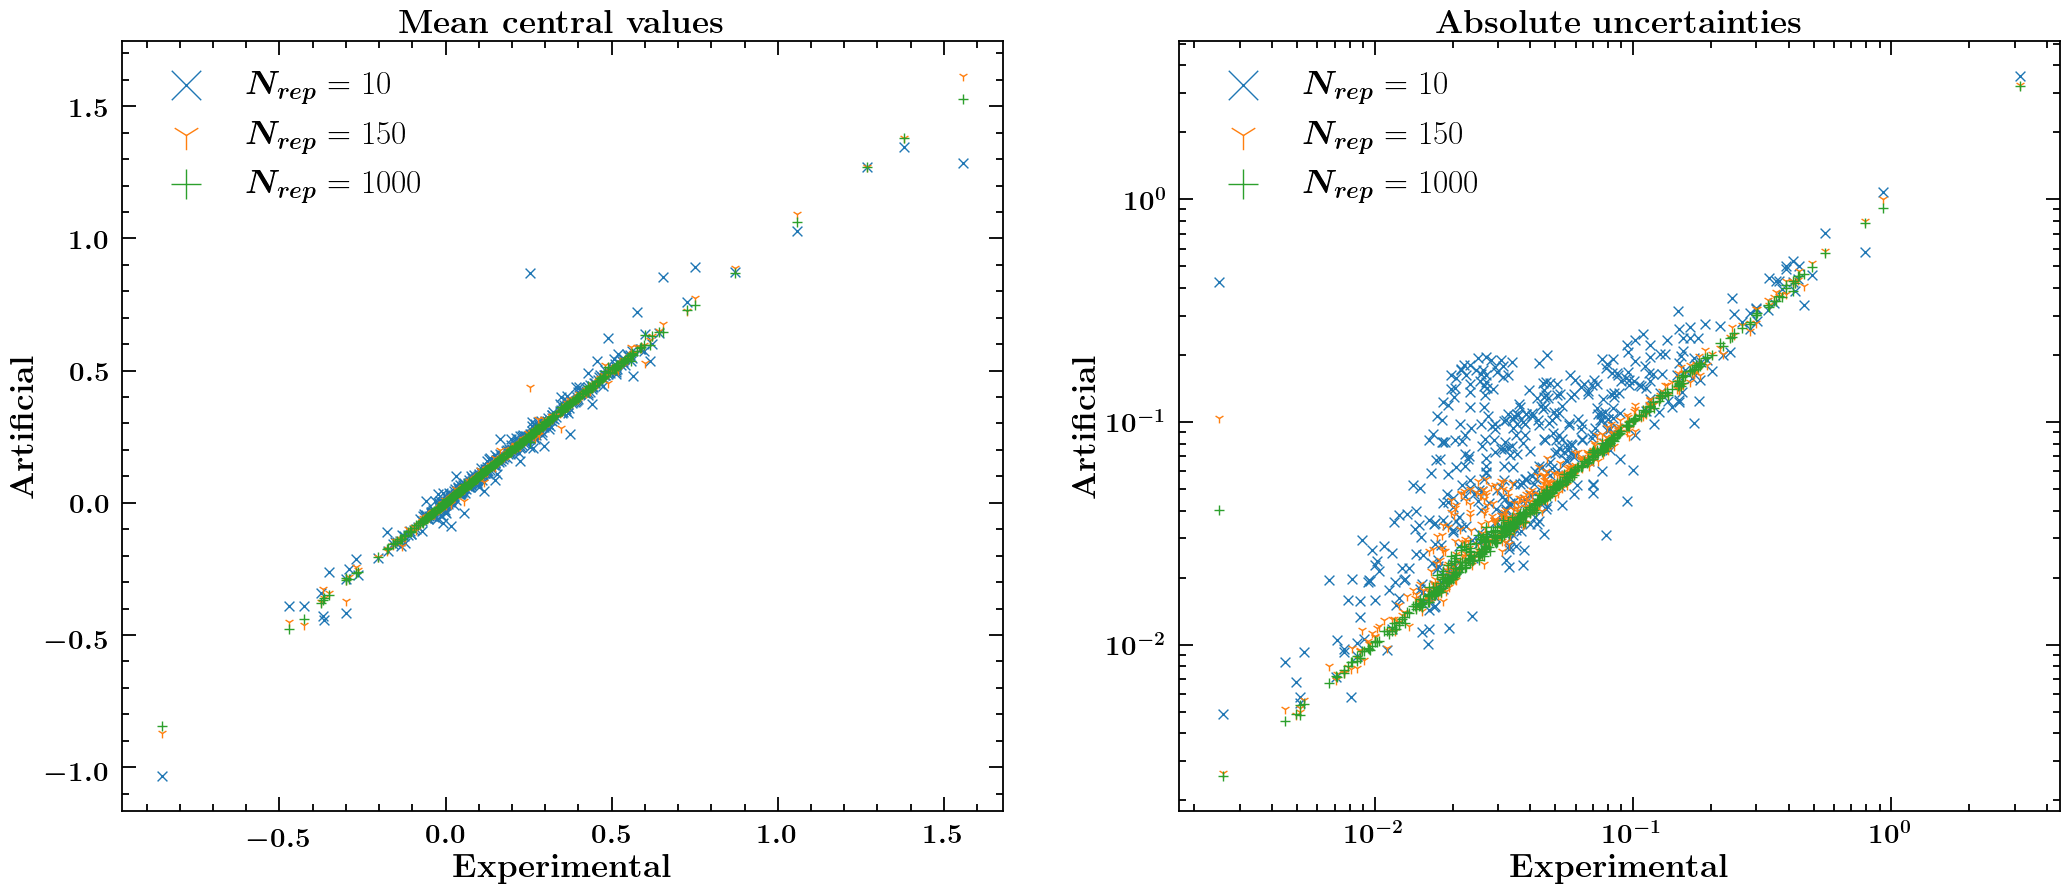
\includegraphics[width=1\textwidth]{replica_number.png } 
    \caption{\small{Scatter plot of experimental versus artificial Monte Carlo mean central values and absolute uncertainties of polarized structure functions computed from ensembles made of $N_{\T{rep}} = 10$, $100$, $1000$ replicas.\\}
    \vspace{1cm}}
    \label{fig:replica_number}
  \end{figure}
  %%
  \begin{table}[!h]
    \scriptsize
    \centering % Center table
    \begin{tabular}{lccc@{\hspace{1cm}}ccc}
  \toprule \toprule
   Experiment    & \multicolumn{3}{c}{$\left< \T{PE} \left[ \left<F^{\T{(art)}} \right>  \right] \right> [\%]$} & \multicolumn{3}{c}{$r \left[ F^{\T{(art)}} \right]$}\\[10pt]
  \toprule
                      &    10     &     150   &    1000  &    10     &     150   &    1000  \\
  \midrule
      COMPASS-P $K^-$   &   24.1    &     4.6   &    4.2   &  .96321  &  .99928  &  .99986 \\
      COMPASS-P $K^+$   &    3.8    &     0.9   &    0.8   &  .99829  &  .99996  &  .99992 \\
    COMPASS-P $\pi^-$   &    5.0    &     1.0   &    0.4   &  .99824  &  .99945  &  .99997 \\
    COMPASS-P $\pi^+$   &    4.9    &     0.7   &    0.1   &  .99916  &  .99993  &  .99999 \\
      COMPASS-D $K^-$   &   41.3    &    14.5   &    3.6   &  .81885  &  .99071  &  .99740 \\
      COMPASS-D $K^+$   &    4.4    &     0.8   &    0.3   &  .98961  &  .99958  &  .99990 \\
    COMPASS-D $\pi^-$   &    9.1    &     1.2   &    0.5   &  .99187  &  .99955  &  .99999 \\
    COMPASS-D $\pi^+$   &    3.8    &     0.8   &    0.5   &  .99538  &  .99991  &  .99997 \\
      HERMES-D  $K^-$   &   10.4    &     1.4   &    0.6   &  .99724  &  .99994  &  .99996 \\
      HERMES-D  $K^+$   &    1.9    &     0.5   &    0.2   &  .99841  &  .99995  &  .99998 \\
    HERMES-D  $\pi^-$   &    2.8    &     0.9   &    0.2   &  .98590  &  .99877  &  .99998 \\
    HERMES-D  $\pi^+$   &    3.1    &     0.6   &    0.2   &  .99641  &  .99980  &  .99998 \\
    HERMES-P  $\pi^-$   &    1.0    &     0.2   &    0.1   &  .99608  &  .99657  &  .99986 \\
    HERMES-P  $\pi^+$   &    0.5    &     0.1   &    0.0   &  .99389  &  .99996  &  .99999 \\
               E143-D   &    2.6    &     0.8   &    0.3   &  .98091  &  .99891  &  .99988 \\
               E143-P   &    0.4    &     0.2   &    0.0   &  .99927  &  .99978  &  .99999 \\
               E154-N   &    0.9    &     0.2   &    0.1   &  .99346  &  .99987  &  .99996 \\
               E155-P   &    0.4    &     0.1   &    0.1   &  .99912  &  .99984  &  .99987 \\
               E155-N   &   10.8    &     1.7   &    0.8   &  .91095  &  .98952  &  .99951 \\
                EMC-P   &    0.6    &     0.3   &    0.0   &  .99228  &  .99775  &  .99994 \\
         JLAB E06 014   &    4.7    &     0.4   &    0.1   &  .97261  &  .99955  &  .99997 \\
         JLAB E97 103   &    0.1    &     0.0   &    0.0   &  .99944  &  .99968  &  .00000 \\
         JLAB E99 117   &    0.2    &     0.0   &    0.0   &  .99605  &  .99979  &  .99993 \\
      JLAB EG1 DVCS-D   &    0.6    &     0.2   &    0.1   &  .99855  &  .99990  &  .99999 \\
      JLAB EG1 DVCS-P   &    0.2    &     0.1   &    0.0   &  .99979  &  .99998  &  .00000 \\
                SMC-D   &    0.8    &     0.2   &    0.1   &  .97954  &  .99434  &  .99973 \\
                SMC-P   &    0.2    &     0.1   &    0.0   &  .99522  &  .99918  &  .99980 \\
            COMPASS-P   &    0.2    &     0.1   &    0.0   &  .99747  &  .99899  &  .99976 \\
             HERMES-N   &    0.8    &     0.1   &    0.1   &  .99377  &  .99971  &  .99987 \\
             HERMES-D   &    0.5    &     0.1   &    0.0   &  .99562  &  .99929  &  .99991 \\
             HERMES-P   &    0.1    &     0.0   &    0.0   &  .99854  &  .99985  &  .99999 \\
  \midrule \bottomrule
\end{tabular}
    \caption{
      \small
      Table of statistical estimators for the mean value computed from the Monte Carlo sample with $N_{\T{rep}}=10,\, 150,\, 1000$ replicas.
    \label{tab:PE}}% Add 'table' caption
  \end{table}
  \clearpage
}
%
The number of replicas is chosen in order to faithfully reproduce the statistical estimators of the original experimental data. For instance, we can check if the averages and the variances of the replica sample, that is
%%
\begin{equation}
  \langle F_{i}^{\T{(art)}} \rangle = \frac{1}{N_{\T{rep}}} \sum_{k=1}^{N_{\T{rep}}} F_{i}^{(k)} \hspace{5mm} \T{and} \hspace*{5mm} \sigma_i^{\T{(art)}} = \sqrt{ \langle \left( F_{i}^{\T{(art)}} \right) \rangle - \langle F_{i}^{\T{(art)}} \rangle^2} \,,
\end{equation}
%%
reproduce the experimental central values and the uncertainties. Such a comparison is shown in Fig.~\ref{fig:replica_number}, where we display scatter plots of the central values and errors for sample of $N_{\T{rep}} = 10$, $150$ and $1000$ replicas. Although they only provide a qualitative description, they clearly show that the accuracy of the sample increases with the size of the Monte Carlo sample. A more quantitative description can be carried out by defining appropriate statistical estimators. Following Ref.~\cite{DelDebbio:2004xtd}, we use the percentage error and the scatter correlation r for central values, whose definitions are
%
\begin{gather}
  \left< PE \left[ \left< F^{(\T{art})} \right>_{\T{rep}} \right] \right>_{\T{dat}} = \frac{1}{N_{\T{dat}}} \sum_{i=1}^{N_{\T{dat}}} \frac{\abs{\left< F_i^{\T{(art)}} \right>_{\T{rep}} - F_{i}^{\T{(exp)}}}}{F_i^{\T{(exp)}}}\,, \\
  r \left[ F^{\T{(art)}} \right] = \frac{\left< F^{\T{(exp)}} \left< F^{\T{(art)}} \right>_{\T{rep}} \right>_{\T{dat}} - \left< F^{\T{(exp)}} \right>_{\T{dat}} \left<  \left< F^{\T{(art)}} \right>_{\T{(rep)}}\right>_{\T{dat}} }{\sigma_s^{\T{(exp)}} \sigma_s^{\T{(art)}} }\,,
\end{gather}
%%
where the scatter variance are defined as
%%
\begin{gather}
  \sigma^{\T{(exp)}}_s = \sqrt{\left< \left( F^{\T{(exp)}} \right)^2 \right>_{\T{dat}} - \left( \left< F^{\T{(exp)}} \right>_{\T{dat}} \right)^2} \,,\\
  %
  \sigma^{\T{art}}_s = \sqrt{\left< \left( \left<F^{\T{(art)}}\right>_{\T{rep}} \right)^2 \right>_{\T{dat}} - \left( \left< \left<F^{\T{(art)}}\right>_{\T{rep}} \right>_{\T{(dat)}} \right)^2} \,.
\end{gather}
%%
Essentially, the percentage error describes how well the central values are recovered by the Monte Carlo sample. On the other hand, the scatter correlation $r$ reflects the capacity of the Monte Carlo sample to reproduce the correlations that are present in the original data set. For each experiment, we show these two values for the observables $g_1^{(h)}$ and $g_1^{(h)}/F_1^{(h)}$ in Tab.~\ref{tab:PE}. We see that a Monte Carlo sample with size $N_{\T{rep}} = 150$ gives a satisfactory reproduction of mean values and uncertainties of experimental data. The improvements obtained by using a larger sample are moderate, and, in any case, do not justify the higher computational effort. For these reasons, we will henceforth adopt the ensemble with $N_{\T{rep}} = 150$ replicas as the standard configuration for our fits.

%_________________________________
\section{Details of the analysis}
\label{sec:4.2}
Here we summarise the aspects concerning the QCD analysis of polarised structure functions. The main observables throughout the analysis are the structure functions $g_1$, Eq.~\eqref{eq:g1_QFT}, and $g_1^h$, Eq.~\eqref{eq:g1h}, for DIS and SIDIS respectively. They are expressed in terms of combinations of PDFs and provide complementary constraints on the distributions.%

On the one hand, data coming from DIS experiments constraints only the linear combination of $\Delta \Sigma$, $\Delta T_3$, $\Delta T_8$, together with $\Delta g$, as it can be easily seen from Eq.~\eqref{eq:g1_NPM_ev}. On the other hand, SIDIS data provides full flavour separation. Moreover, given that data with kaons in the final state are given, the constraining power for the strange distributions $\Delta s$ and $\Delta \bar{s}$ is strengthened. In both SIDIS and DIS processes, the gluon distribution $\Delta g$ is weakly constrained. Indeed, it enters at NLO and its effect is lessened by the running coupling. Processes other than those we have just discussed (such as jet or semi-inclusive production in proton-proton collisions), receiving LO contributions from gluon initiated subprocesses, may provide direct information on the gluon distribution \cite{Rojo:2015acz}.%

Since we use data with different targets, we must take into account the hadron that PDFs refer to. The proton, neutron, and deuteron PDFs are related to each other by isoscalarity (assumed as an exact symmetry) so that
%%
\begin{equation}
  \begin{split}
    &\Delta u^{(I)} = I \Delta u^p + ( 1 - I ) \Delta d^p \\
    &\Delta d^{(I)} = I \Delta d^p + ( 1 - I ) \Delta u^p
  \end{split}
  \label{eq:iso_rel}
\end{equation}
%%
where $I=1$, $0.5$ and $0$ representing proton, deuteron, and neutron respectively. A similar relation also holds for antiquark distributions. We will henceforth assume that PDFs refer to the proton. The other distributions can be obtained by means of Eqs.~\eqref{eq:iso_rel}.%

Since both $\Delta s$ and $\Delta \bar{s}$ are sea-distributions for all targets, we will further assume that
%%
\begin{equation}
  \Delta s = \Delta \bar{s} \,.
\end{equation}
%%
In doing so, we decrease the number of unknown quantities, and focus the analysis to valence quarks. We will also neglect the heavier quark and antiquark distributions for charm and bottom flavours. The threshold under which this assumption is reliable has been fixed to the quark masses, assuming the values $m_c=1.51\, \T{GeV}$ and $m_b=4.92\, \T{GeV}$. For the QCD calculation, the value for the strong coupling constant has been fixed to $\alpha_s(M_Z^2) = 0.118$.\par
Finally, the computation of SIDIS observables requires the introduction of fragmentation functions sets. For this analysis, we will use the pion and kaon fragmentation functions sets \texttt{MAPFF1.0} obtained from a global analysis carried out at next-to-next-to-leading order \cite{Khalek:2021gxf, AbdulKhalek:2022laj}.

\section{Fitting configuration}
\label{sec:4.3}
In this section, we shall give the details of the fitting configuration adopted in the \texttt{MAPPol1.0} analysis. We discuss which flavours are taken into account and how the distributions are parametrised in terms of neural network. Then, we will move to the description of the training procedure, providing a more detailed picture than that given in \secref{sec:NNtr}. In particular, we will see the difference between the error function used during the minimisation and the global error function. Finally, we review the theoretical constraints assumed in the analysis and their implications.

\subsection*{Neural Network parametrisation}
The six independent distributions that are of our concern throughout the analysis are $\Delta u, \, \Delta d, \, \Delta s, \, \Delta \bar{u}, \, \Delta \bar{d}$ and $\Delta g$. These distributions are parametrised in terms of a single multi-layer feed-forward neural network, whose output layer is compounded of six differential nodes, one for each distribution. The PDFs are intended to be parametrised at an initial scale $\mu_0 = 1 \, \T{GeV}$. The output of the network is then evolved to the experimental scale by means of the DGLAP equations, Eq.~\eqref{eq:DGLAP_coupled}.%

The architecture of the neural network is 1-10-6, which entails 86 free parameters. We explicitly verified the parametrisation to be redundant, ensuring that the results do not depend on the architecture. Indeed, keeping on the single deep-layer structure, we have not observed any considerable differences in the results by either improving the nodes of the internal layer up to 20 or reducing this number to 5. We figured out that an architecture with 10 internal nodes is a good compromise between the number of parameters and the redundancy in the parametrisation, which is enough to reproduce any functional form given sufficient training time.%

The single node in the input layer corresponds to the Bjorken variable $x$. Other determinations supplement the above parametrisation with a preprocessing function. This consists of multiplying the neural network by a fixed function that reflects some known behaviour of the distributions. For instance, the \texttt{NNODFpol1.0} analysis from NNPDF collaboration \cite{Nocera:2014gqa} introduces these functions to implement small- and large-x behaviours of the distributions. Even though such an approach may help the algorithm in terms of efficiency, it can be source of biases. For that reason, we choose to use the neural network without any preprocessing function.%

All the nodes except for the input node use a sigmoid as activation function, Eq.~\eqref{eq:sigmoid}. However, we slightly modify the outputs of the last node in order to constraint to zero parton distributions at $x=1$ and to implement, analytically, theoretical constraints, as we shall see later.%

Finally, we remark that there are as many networks as the number of replicas that we are working with. In our case, we will deal with 150 neural networks, representing the statistical ensemble of polarised PDFs. Since dealing with such a huge number of networks is a heavy computational task, the outputs (\textit{i.e.}, the PDFs) are put on a grid in the $(x,Q^2)$ plane. The value for an arbitrary pair $(x,Q^2)$ can be easily accessed through the LHAPDF interface \cite{Buckley:2014ana}. A schematic representation of the neural network and of the subsequent steps is sketched in Fig.~\ref{fig:NN_plot}.
%%
\begin{figure}[t]
  \centering
  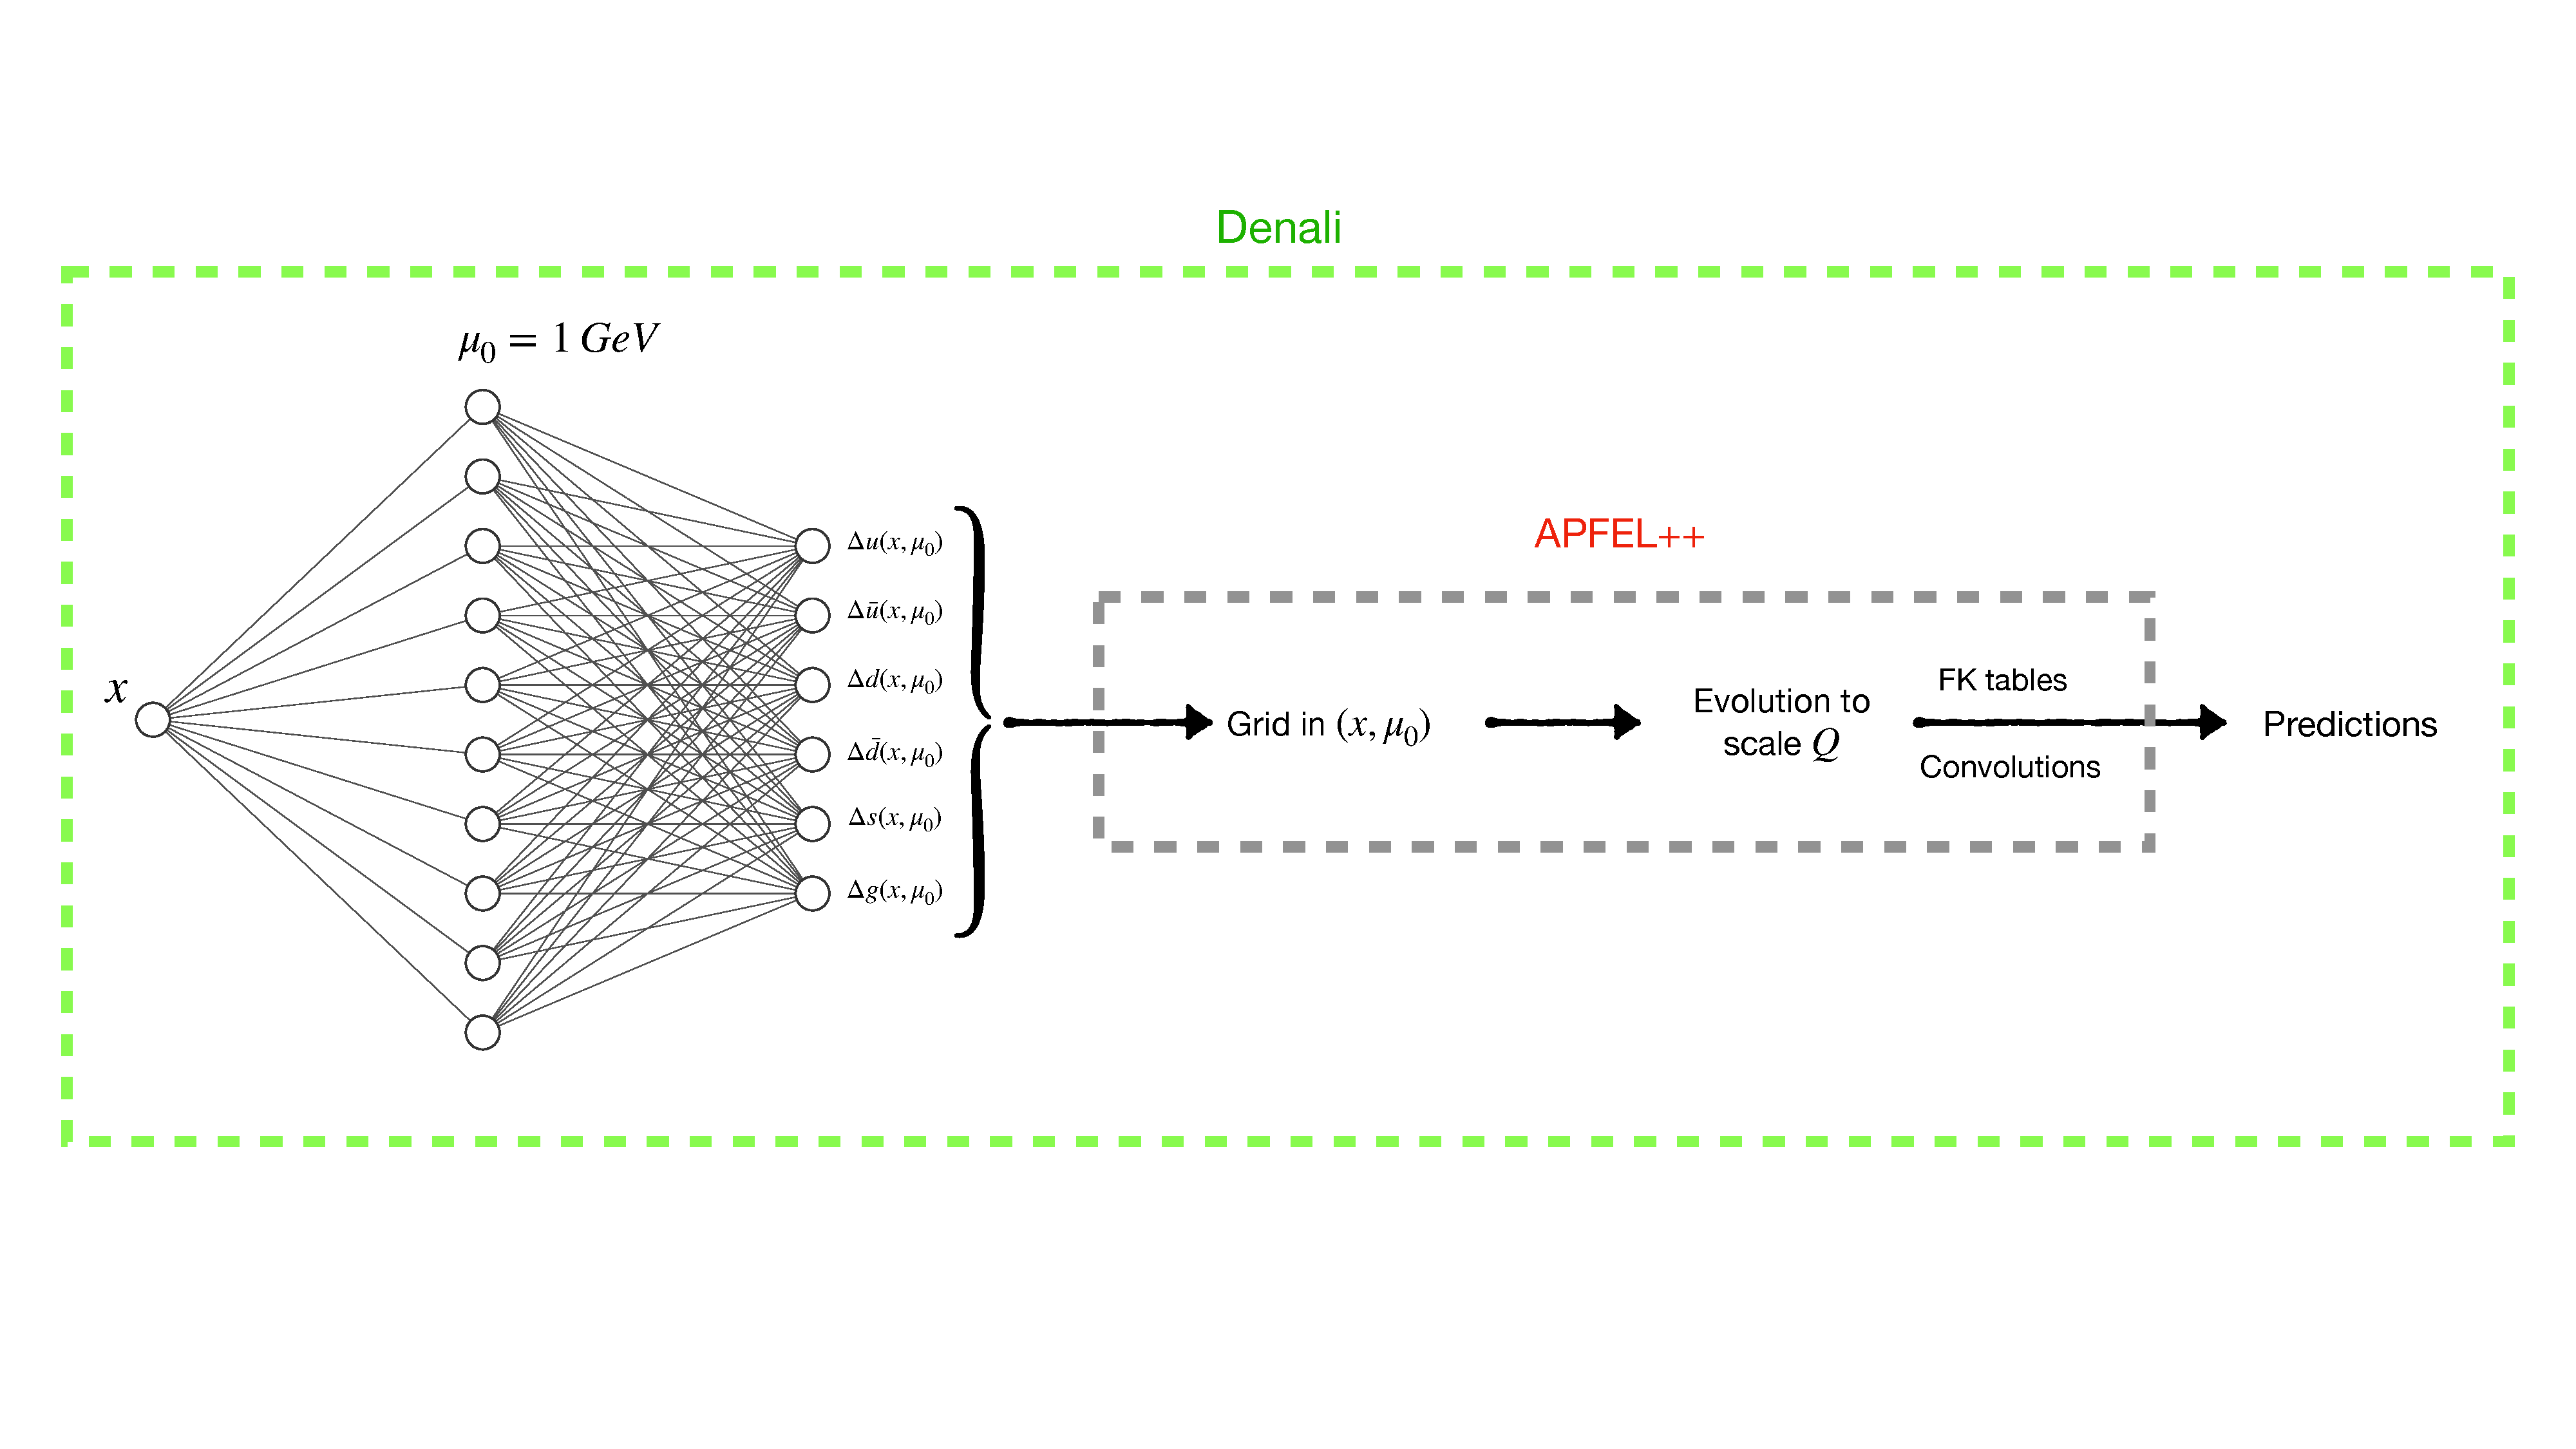
\includegraphics[width=1\textwidth]{NN_plot.pdf} 
  \caption{\small{Scheme of the \texttt{Denali} algorithm.}}
  \label{fig:NN_plot}
\end{figure}
%%

\subsection*{Optimization and determination of the optimal fit}
Optimization is the process where the parameters are optimised through the minimisation of the figure of merit over the parameter space. Each replica of the ensemble (\textit{i.e.}, each network) undergoes an independent optimisation procedure. Although this process can be computationally expensive if a high number of replicas is used, we can use parallel processing methods, and the time required by a single global fit is considerably reduced.%

The figure of merit for the $k$-th replica is defined as
%%
\begin{equation}
  E^{(k)} = \frac{1}{N_{\T{dat}}} \sum_{i,j}^{N_{\T{dat}}} \left( g_{i}^{\T{(art)}(k)} - g_{i}^{\T{(net)}(k)} \right) (\T{cov})^{-1}_{ij} \left( g_{j}^{\T{(art)}(k)} - g_{j}^{\T{(net)}(k)} \right) \,.
  \label{eq:EF_k}
\end{equation}
%%
The above expression requires few comments. The observable $g_{i}^{\T{(art)}(k)}$ is the $k$-th Monte Carlo replica of the $i$-th data point, whereas $g_{i}^{(net)(k)}$ is its prediction provided by the $k$-th neural network representing the $k$-th replica of the PDF ensemble. Finally, $\T{(cov)}$ is the usual covariance matrix constructed from the experimental sets.%

The error function, Eq.~\eqref{eq:EF_k}, must not be confused with the $\chi^2$ used to quantify the goodness of the final result. Indeed, it can be shown that Eq.~\eqref{eq:EF_k} does converge to $2$ instead of $1$. The reason being that the prediction is compared against the fluctuated data and not against the experimental central value. The quantity we should refer to as the $\chi^2$ involves 
experimental central value and is defined as
%%
\begin{equation}
  \chi^2 = \frac{1}{N_{\T{dat}}} \sum_{i,j}^{N_{\T{dat}}} \left( F_{i}^{\T{(exp)}} - \left<F_{i}^{\T{(net)}}\right>_{\T{rep}} \right) (\T{cov})^{-1}_{ij} \left( F_{j}^{\T{(art)}} - \left<F_{j}^{\T{(net)}}\right>_{\T{rep}} \right) \,,
  \label{eq:global_chi2}
\end{equation}
%%
where the average over replicas is defined as
%%
\begin{equation}
  \left< F_i^{\T{(net)}} \right>_{\T{rep}} = \frac{1}{N_{\T{rep}}} \sum_{k} F^{(k)}_i \,.
\end{equation}
%%
Here, $F_i$ may represent one of the observable presented in Tabs.~[\ref{tab:DIS_data},\ref{tab:SIDIS_data}]. We will refer to Eq.~\eqref{eq:global_chi2} as the global $\chi^2$. It is computed at the end of the optimisation procedure and thus it is not minimised. The parameter space is explored with the SGD method discussed in \secref{sec:NNtr}, which sought for the minimum of the error function, Eq.~\eqref{eq:EF_k}.%

As discussed at the end of \secref{sec:NNtr}, the neural network parametrisation is able to fit not only the underlying physics, but also statistical noise of the data set -- a problem also known as \textit{overlearning}. Thus, the best fit does not always coincide with the minimum of the figure of merit, Eq.~\eqref{eq:EF_k}. In order to find the best fit, we use the cross-validation method \cite{pml1Book}. It works as follows:
%%
\begin{enumerate}
  \item For each replica, the data sets are randomly divided into two sets -- training and validation sets. They include a fraction $f_{\T{tr}}$ and $f_{\T{val}} = 1 - f_{\T{tr}}$ of the data points, respectively.
  \item During the optimisation procedure, the error function, Eq.~\eqref{eq:EF_k}, is separately computed over the training and the validation set. The former undergoes the minimisation procedure, while the latter is only monitored and not minimised.
  \item Finally, the best fit corresponds to the minimum of the validation's error function within a fixed number of iterations, which in our case corresponds to $N_{\T{iter}} = 3000$.
\end{enumerate}
%%
The profile of the figure of merit for an arbitrary replica is shown in Fig.~\ref{fig:profile}. We see that immediately after the minimum of the validation curve has been reached, it starts to increase, whereas the training curve keeps reducing. This means that the network is learning the statistical noise of the training set, which is different from that of the validation set. In the present analysis, equal training and validation fractions are chosen, that is $f_{\T{tr}} = f_{\T{val}} = 50\%$. However, some experimental sets are highly affected by the kinematic cuts and only a small portion of data points survives. In this case, the training set would be too small, affecting the stability of the minimisation. Hence, if the number of points after cuts is less or equal to 5, all the points will be included in the training set.

%%
\begin{figure}[t]
  \centering
  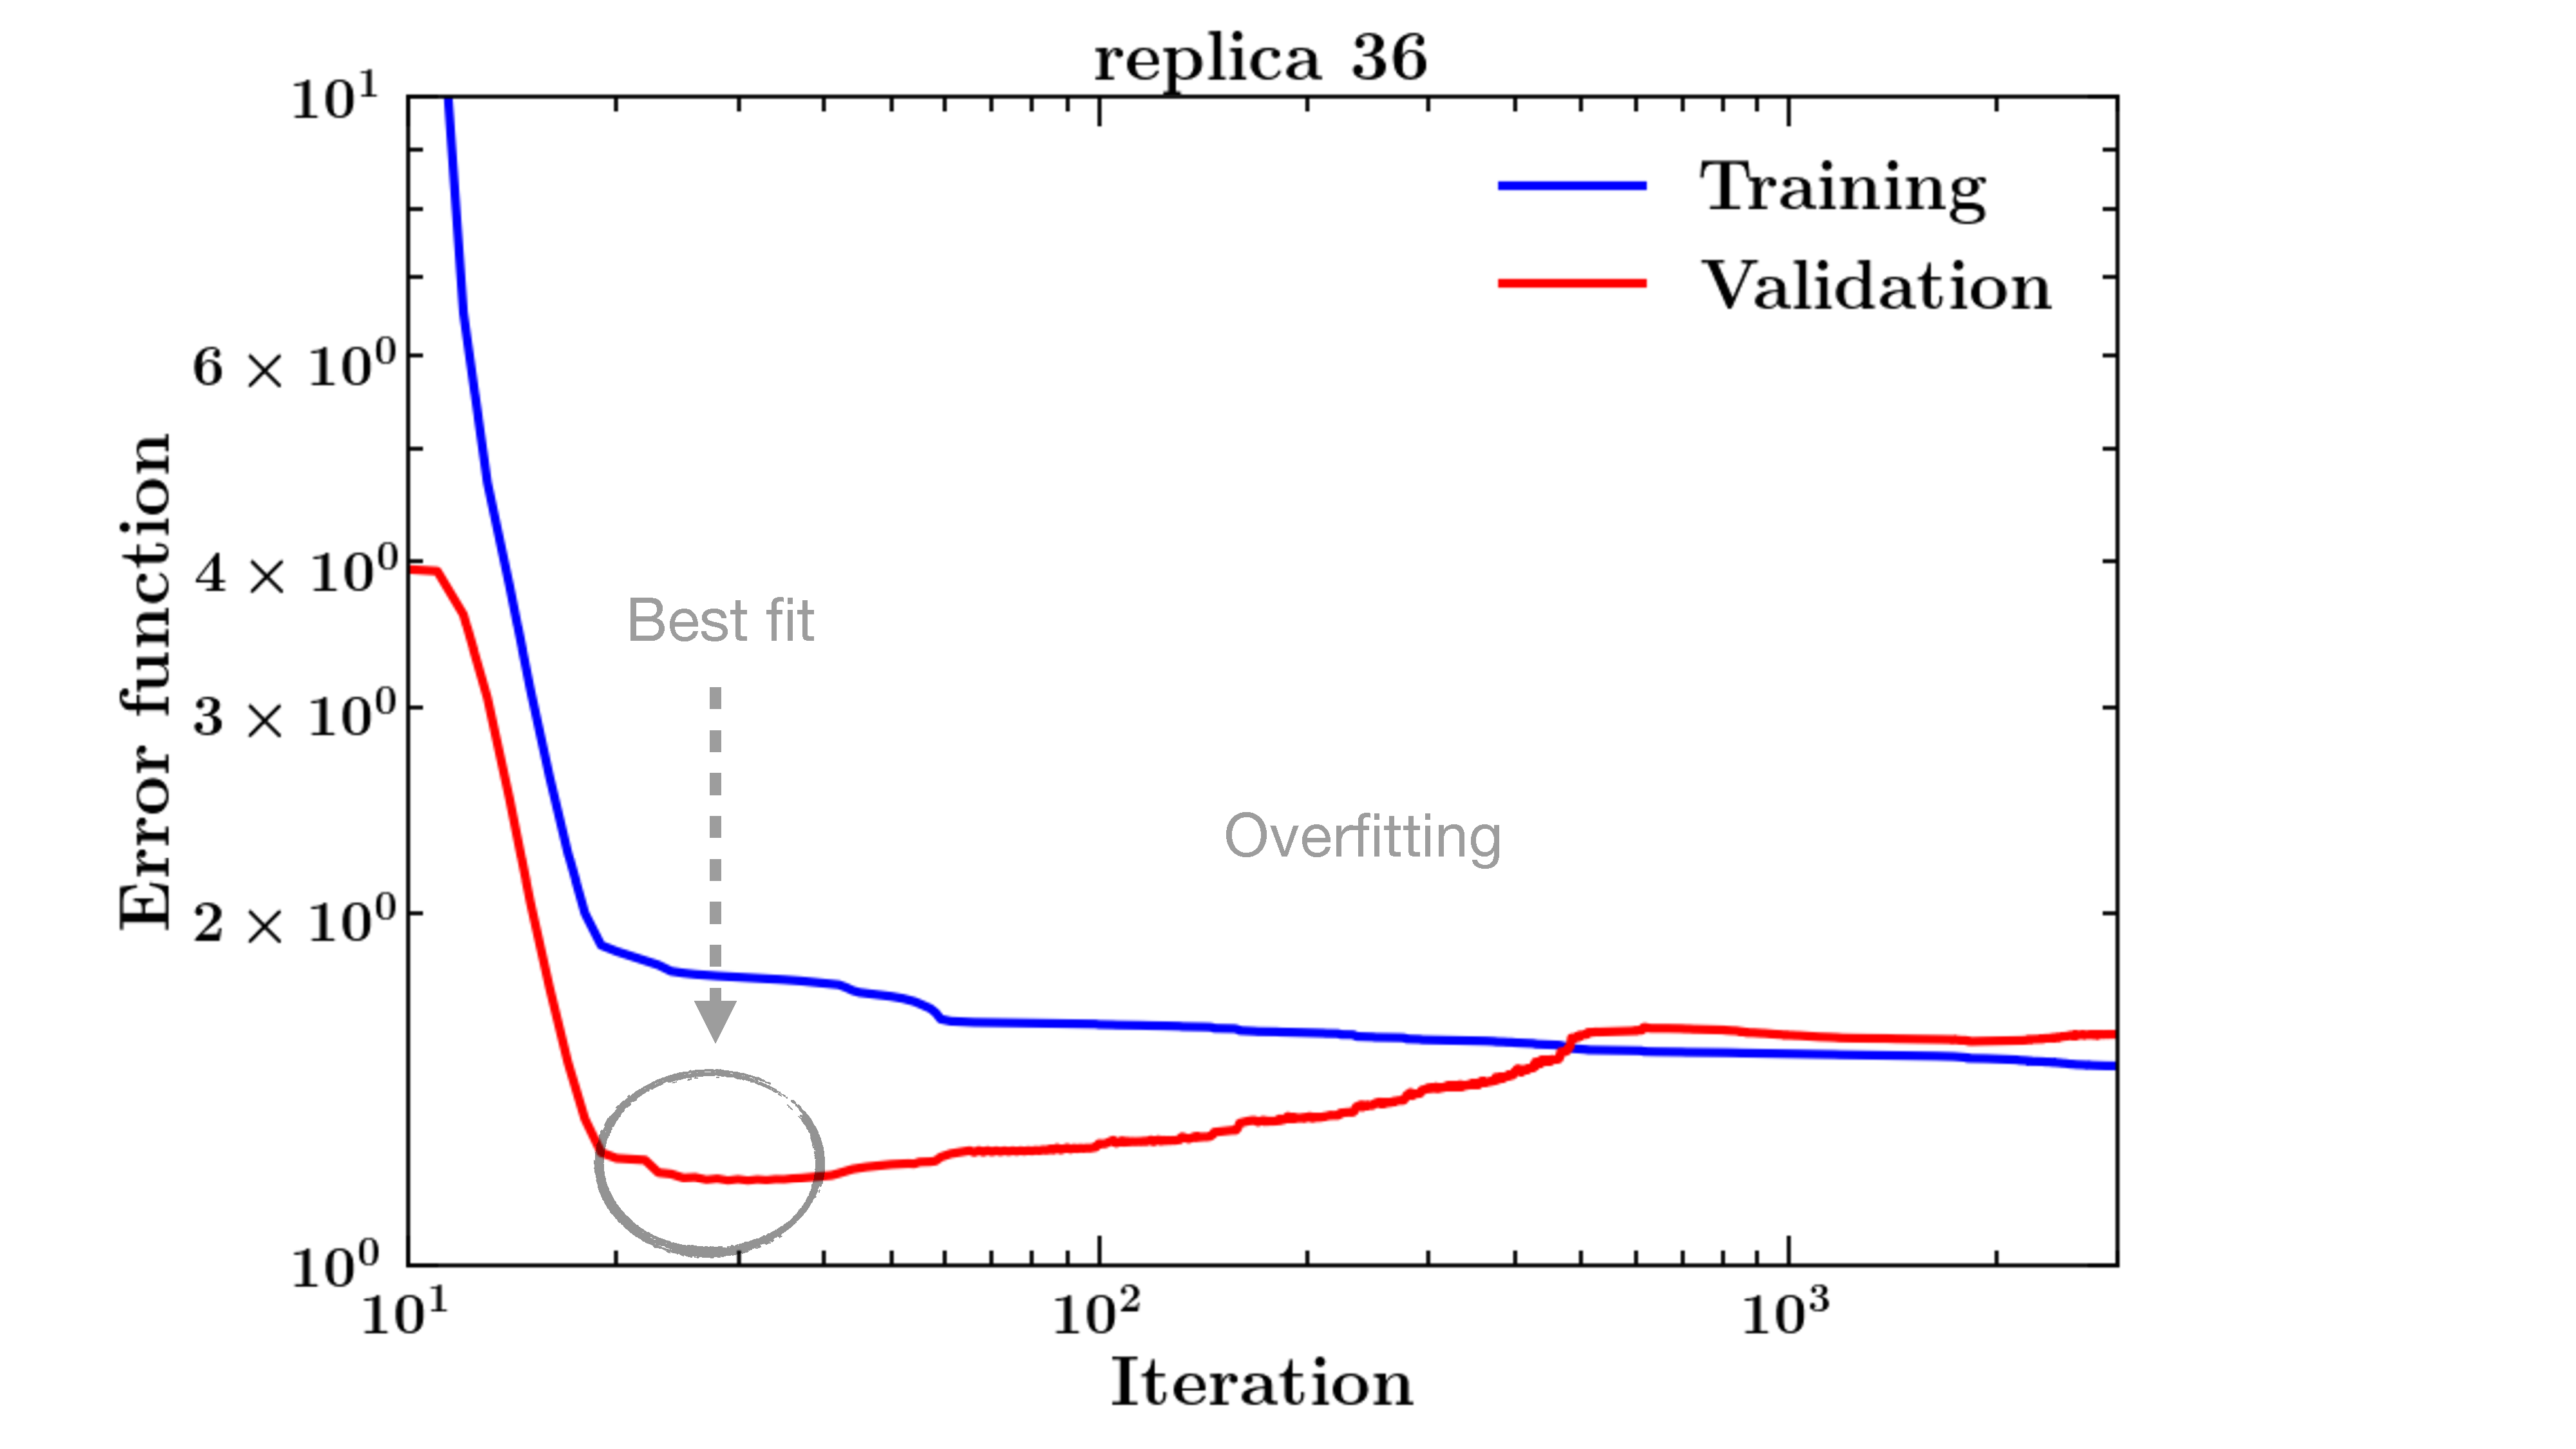
\includegraphics[width=0.6\textwidth]{profile.pdf} 
  \caption{\small{Profile of the error function for the 36th replica. The blue and red curves represent the error as a function of the iteration step for the training and validation steps, respectively.}}
  \label{fig:profile}
\end{figure}
%%

\subsection*{Theoretical constraints}
We have already mentioned that, due to the scarcity and the low accuracy of data, polarised PDF are loosely constrained. This not only affects the efficiency of the algorithm, but has a huge impact on the final result. In order to improve the constraining power and to reduce the uncertainties of the polarised PDFs, we apply theoretical constraints to the analysis. In particular, we consider sum rules and positivity.%

Sum rules refer to the hadronic matrix elements $a_3$ an $a_8$, whose values can be extracted from measurements in hyperon $\beta$-decay, Eqs.~\eqref{eq:a3_a8_values}. They can be related to the PDFs via Eqs.~[\ref{eq:a3_PM}-\ref{eq:a8_PM}], provided that exact $SU(3)_f$ symmetry is assumed. The theoretical constraint is introduced at a data set level. This means that the values in \eqref{eq:a3_a8_values} are treated as standard data points, with central value and (uncorrelated) uncertainty. Hence, at each iteration of the optimisation procedure, the algorithm will compute, in addition to the observable $g_1^{(h)}$ or $g_1^{(h)}/F_1^{(h)}$, the predictions for $a_3$ and $a_8$ via Eqs.~[\ref{eq:a3_PM}-\ref{eq:a8_PM}]. Sum rules provide further information on polarised PDFs. If the SIDIS data sets were not included, the only source of information for the sea-quark flavour $\Delta s$ would only come from this theoretical constraint. It will be interesting to study how these constraints affect that distribution if SIDIS data sets are excluded.%

The other theoretical constraints, which enforce the most the PDFs, is the positivity constraint. The key point is that the cross-sections that enter the polarised asymmetries, Eq.~\eqref{eq:asymmetry}, must be positive. This implies that $g_1^{(h)}$ is bounded by its unpolarised counterpart $F_1^{(h)}$, that is
%%
\begin{equation}
  \begin{split}
    \left| g_1 (x,Q^2)  \right|& \leq F_1(x, Q^2) \,,\\
    \left| g_1^{(h)} (x,z,Q^2)  \right|& \leq F_1^{(h)}(x, z, Q^2) \,.
  \end{split}
  \label{eq:positivity_obs}
\end{equation}
%%
Given that at leading order the structure function are proportional to parton distributions, and that Eq.~\eqref{eq:positivity_obs} must be satisfied for any choice of target (\textit{i.e.}, for any combination of quark plus antiquarks), it must be satisfied by each flavour separately. Hence, at leading order, we have
%%
\begin{equation}
  \left| \Delta f_i (x,Q^2) \right| \leq f_i (x,Q^2) \,,
  \label{eq:positivity_fl}
\end{equation}
%%
for all $x$ and for all $Q^2$, being $f_i$ the relative unpolarised PDF set. At NLO and beyond the positivity constraint, Eq.~\eqref{eq:positivity_fl}, receives perturbative corrections. Nevertheless, it can be shown \cite{Altarelli:1998gn} that, even at relatively small values down to $Q^2 \sim 1 \, \T{Gev}^2$, the modified positivity bounds for each flavours are slightly different from the leading order bounds, and the difference between LO and higher orders is negligible. Moreover, the positivity bound exhibits his constraining effects only at large x, where the higher order corrections to the LO positivity bound are lessened. Imposing positivity bounds consistently guarantees positivity of physical cross-sections.%

The positivity bound Eq.~\eqref{eq:positivity_fl} must take into account the uncertainties of the unpolarised PDFs. This problem can be addressed with two different solutions. The first imposes the leading-order bound Eq.~\eqref{eq:positivity_fl} by requiring
%%
\begin{equation}
  \left| \Delta f_i (x,Q^2) \right| \leq \left<f_i (x,Q^2)\right>_{\T{rep}} + \sigma_i(x,Q^2) \,,
  \label{eq:positivity_fl_sigma}
\end{equation}
%%
where $\left<f_i (x,Q^2)\right>_{\T{rep}}$ is the mean value over the statistical ensemble of unpolarised PDFs and $\sigma_i(x,Q^2)$ its corresponding one-sigma uncertainty, both evaluated at the kinematic point $(x,Q^2)$. This ensures that also the uncertainty of the unpolarised distribution is propagated through the analysis within a standard deviation. On the other hand, the second approach applies the same bound Eq.~\eqref{eq:positivity_fl}, but with randomly chosen replica from the statistical set of distributions. This means that, replica by replica, the unpolarised PDF that enters the constraint is different. Hence, this stocasticity spans the space of distributions, reflecting the uncertainties of the statistical ensemble in the bound. For consistency, the unpolarised PDF set is the same that has been used to compute the unpolarised structure function $F_1^{(h)}$. \red{Which method do we adopt?}%

The positivity constraint is introduced analytically in the present work, acting on the output layer of the neural network. Indeed, for each output node of the last layer (\textit{i.e.}, for each parametrised flavour), we impose
%%
\begin{equation}
  \sigma_{i} (x,\mu_0) \rightarrow \Delta f_{i} (x, \mu_0) \equiv \bigl[ 2 \sigma(x,\mu_0) - 1 \bigr] \, f_{i} (x,\mu_0) \,,
  \label{eq:pos_net}
\end{equation}
%%
being $\sigma_i(x,\mu^2)$ the sigmoid activation function of the $i$-th output of the network. We observe that Eq.~\eqref{eq:pos_net} not only imposes the positivity bound Eq.~\eqref{eq:positivity_fl}, but also constraint to zero parton distribution at $x=1$, provided that the unpolarised PDF is zero at the same point. 

\section{Results}
\label{sec:4.4}

